% \documentclass{book}

\documentclass[12pt]{article}
\usepackage[pdfborder={0 0 0.5 [3 2]}]{hyperref}%
\usepackage[left=1in,right=1in,top=1in,bottom=1in]{geometry}%
\usepackage[shortalphabetic]{amsrefs}%
\usepackage{amsmath}
\usepackage{enumerate}
\usepackage{enumitem}
\usepackage{amssymb}                
\usepackage{amsmath}                
\usepackage{amsfonts}
\usepackage{amsthm}
\usepackage{bbm}
\usepackage[table,xcdraw]{xcolor}
\usepackage{tikz}
\usepackage{float}
\usepackage{booktabs}
\usepackage{svg}
\usepackage{mathtools}
\usepackage{cool}
\usepackage{url}
\usepackage{graphicx,epsfig}
\usepackage{makecell}
\usepackage{array}

\def\noi{\noindent}
\def\T{{\mathbb T}}
\def\R{{\mathbb R}}
\def\N{{\mathbb N}}
\def\C{{\mathbb C}}
\def\Z{{\mathbb Z}}
\def\P{{\mathbb P}}
\def\E{{\mathbb E}}
\def\Q{\mathbb{Q}}
\def\ind{{\mathbb I}}

\begin{document}
\section*{Homework 6}
In this problem, we looked at the function
\[
u(x) = \frac{1}{1 + x^2}
\]
on the interval $[-1, 1]$. We then performed an interpolation of this function using Legendre and Chebyshev polynomials. We used $N$ interpolation points, and the points chosen were the Gaussian quadrature points (i.e. the endpoints of the interval were not included). For each value of $N$, we computed the discrete $L^2$ error, the continuous $L^2$ error (using Gaussian quadrature on the polynomial interpolant), and the $L^\infty$ error (by evaluating the polynomial interpolant on a fine mesh). The error was measured for both the interpolant and for the derivative of the interpolant, i.e. for:
\begin{enumerate}
	\item $u - I_N u$
	\item $u' - (I_N u)'$
\end{enumerate}

\subsection*{Legende Polynomials}
For the Legendre interpolation, the output and error table is given below.

\begin{figure}[H]
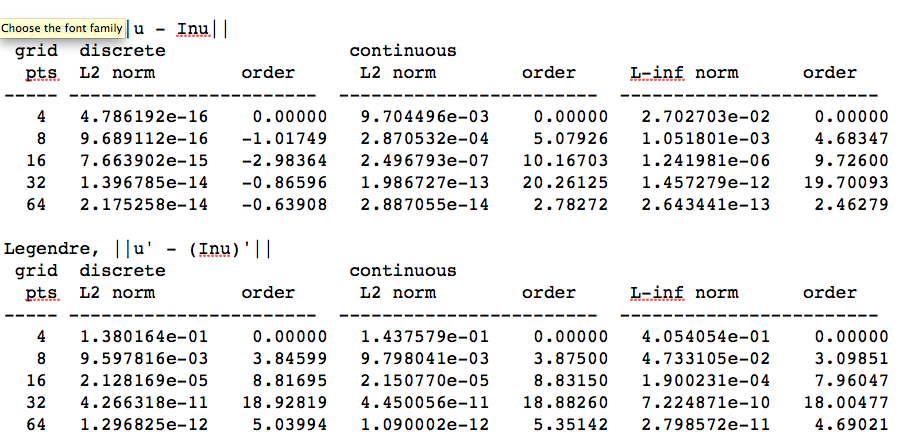
\includegraphics[width=12cm]{images/legendre.png}
\end{figure}

For the discrete $L^2$ error, we are at machine precision for all number of grid points. For the continuous $L^2$ error and the $L^\infty$ error, the order increases with increasing number of grid points until machine precision is reached. This suggests exponential convergence, which is unsuprising since we are interpolating an analytic function. This hold for both the interpolant and the derivative of the interpolant. Error plots on a semi-log scale will be given below.

\subsection*{Legende Polynomials}
For the Chebyshev interpolation, the output and error table is given below.

\begin{figure}[H]
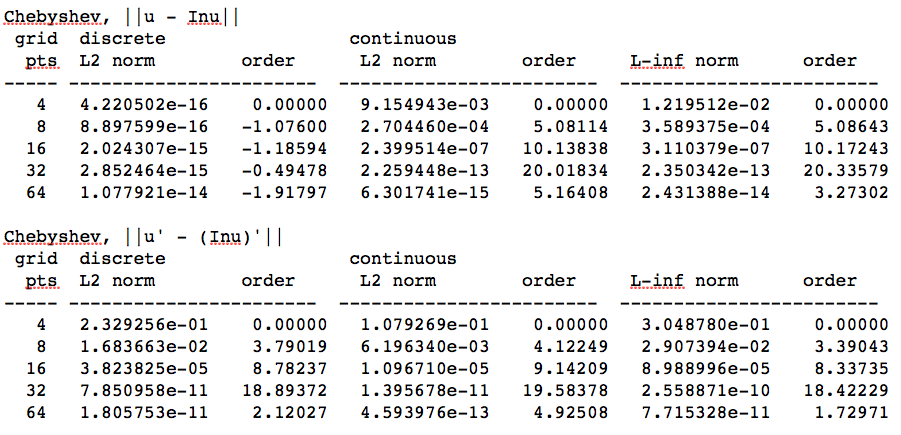
\includegraphics[width=12cm]{images/chebyshev.png}
\end{figure}

For the discrete $L^2$ error, we are again at machine precision for all number of grid points. For the continuous $L^2$ error and the $L^\infty$ error, the order increases with increasing number of grid points until machine precision is reached. This again suggests exponential convergence, which is unsuprising since we are interpolating an analytic function. This hold for both the interpolant and the derivative of the interpolant. Error plots on a semi-log scale will be given below.

\subsection*{Error Plots}

Since the discrete $L^2$ error is at machine precision throughout, we will not give a plot of that error.\\

For the continuous $L^2$ error, we plot the log of the error versus the gridsize. 

\begin{figure}[H]
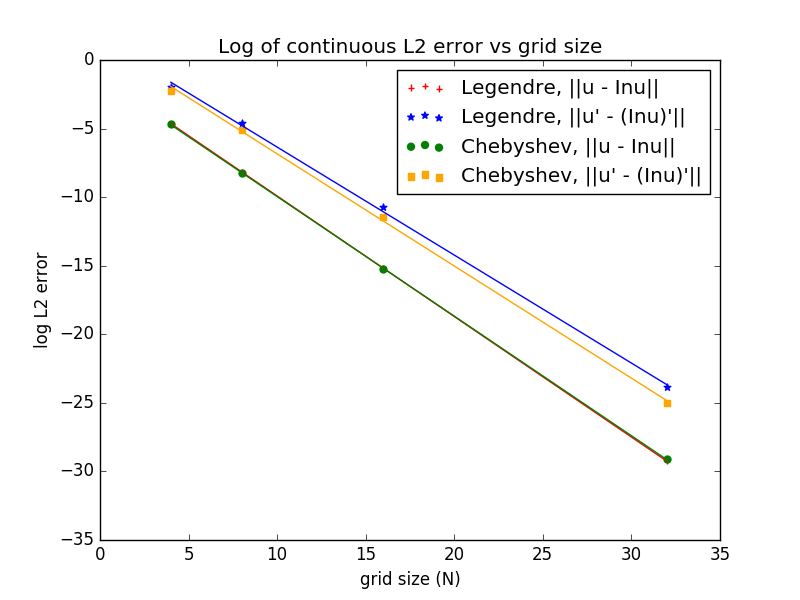
\includegraphics[width=10cm]{images/polyL2error.png}
\end{figure}

In both cases (interpolant and derivative), both types of polynomial interpolation (Legendre and Chebyshev) produce a good best-fit straight line, indicative of exponential convergence. The exponential decay rate is given by the slope of the best-fit straight line.

\begin{figure}[H]
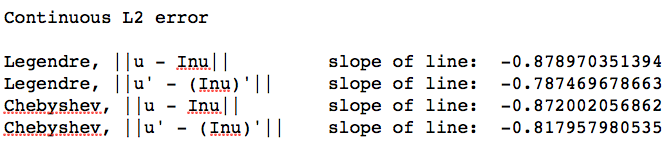
\includegraphics[width=10cm]{images/L2slopes.png}
\end{figure}

For the $L^\infty$ error, we again plot the log of the error versus the gridsize. 

\begin{figure}[H]
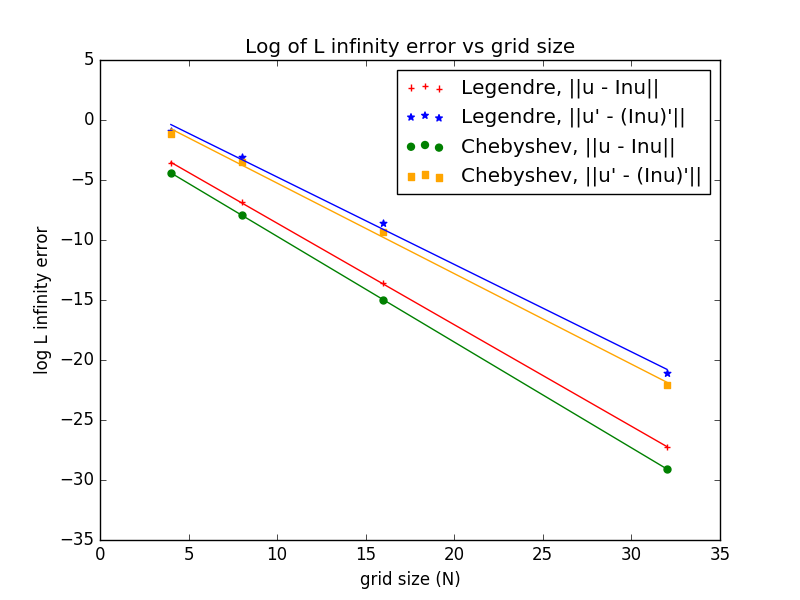
\includegraphics[width=10cm]{images/polyLinferror.png}
\end{figure}

In both cases (interpolant and derivative), both types of polynomial interpolation (Legendre and Chebyshev) also produce a good best-fit straight line, indicative of exponential convergence. The exponential decay rate is given by the slope of the best-fit straight line.

\begin{figure}[H]
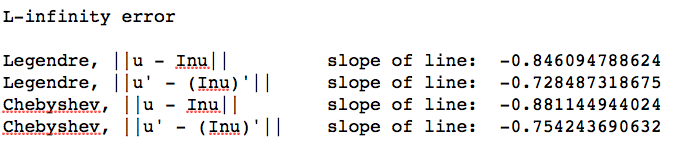
\includegraphics[width=10cm]{images/Linfslopes}
\end{figure}

\end{document}

